\chapter{Marco Teórico - (In) Seguridad en el Browser}
\label{chap3:MT}


En esta sección se presentan los posibles ataques que un \textit{Browser} puede sufrir y que directamente podrían afectar al sistema con el que se comunica. Principalmente ahondaremos en los ataques en el \textit{Browser} relacionados a las técnicas de Ingeniería Social \cite{socEngineeering}. El escenario actual de los ataques en el \textit{browser} ha cambiado bastante, si es comparado a aquellos de la década de los noventa. Cada día los Browsers son más robustos y difíciles de explotar, y por lo mismo los ataques de tipo \textit{drive-by downloads} o los basados en ejecución de código para vulnerar el sistema, cada vez son menores. Una nueva forma de ataque ha emergido y es bastante fácil de lograrlo, pues se basa en el engaño del usuario a realizar lo que el atacante desea. Una vez el usuario es engañado, el atacante puede lograr un control total tanto del \textit{Browser} o del Host, sin haber tenido que vulnerar el sistema \cite{Rajab2013,Labs2013} que aloja al \textit{Browser}. Desarrollos de sistemas críticos que interactuan a diario con diferentes usuarios en la red, deberían de ser los más preocupados de estos ataques, pues atentan contra la confidencialidad, integridad y disponibilidad de los datos, tanto del usuario (personales) como los de los \textit{Stakeholders} involucrados.

\section{Ataques y Amenazas}
Esta sección incluye algunos ataques posibles de realizar en un \textit{Browser} y que podrían afectar tanto directa como indirectamente a un sistema externo. Acá no incluiremos ataques en donde el Host ya ha sido vulnerado con anticipación, o aquellos que puedan correr software con los privilegios de un usuario del sistema Host, es decir, aquellos donde el Host ya ha sido controlado directamente por medio de alguna vulnerabilidad del sistema. En el caso anterior, los Browsers ya nada pueden hacer para detener un ataque de esa magnitud.

En el Top Ten \cite{owaspTopTen} de la OWASP (Open Web Application Security Project) - los diez riesgos de seguridad más importantes en Aplicaciones Web - se puede distinguir en el año 2013 los riesgos directamente relacionados a amenazas de seguridad en el \textit{Browser}. Algunos como: Injección (A1), Manejo de sesiones y autenticación roto (A2), XSS (A3), CSRF (A8) y uso de componentes con vulnerabilidades conocidas (A9), son los riesgos que las organizaciones podrían sufrir en sus sistemas cuando se realizan ciertos ataques en el \textit{Browser}.

En trabajos \cite{barth2008security, FirefoxThreatModel} se puede observar que existen ataques que pueden generar secuelas en otros sistemas, si es que el Navegador es afectado en primera instancia. Algunas amenazas existentes son:

\begin{enumerate}
	\item Compromiso de los componentes del Navegador (plugins incluidos) que poseen privilegios de usuario.
	\item Compromiso del Host/Sistema.
	\item Robo de datos en el tráfico.
	\item Compromiso de páginas web (y su data) de orígenes distintos.
	\item Fijación de sesión o secuestro de ésta.
	\item Compromiso de los canales de comunicación del \textit{Browser}.
\end{enumerate}

\subsection{Social Engineering o Ingeniería Social}
\cite{socEngineeering} define este tipo de acción como: El acto de manipular una persona para realizar acciones que no son parte de los mejores intereses del \textit{blanco o víctima} (la misma persona/organización/etc u otra entidad). Un ataque de éste tipo puede darse de diversas maneras, no dejando la posibilidad de un encuentro físico o digital con el que realiza el engaño. Un ataque basado en ingeniería social, es uno que se aprovecha del comportamiento humano y la confianza de la víctima. En el contexto del Web Browser, el usuario engañado es la primera y última línea de defensa contra este tipo de ataques, pues un abuso en la confianza del usuario podría abrir las puertas al Host del \textit{Browser}, logrando un daño tanto del usuario como con los sistemas externos con los que interactúa.

Si pudieramos dividir los ataques de Social Engineering, podríamos encontrarnos con un panorama parecido al de la Figura \ref{fig:SEattack}. En esta figura es posible observar que los ataques de Clickjacking se encuentran afuera del ámbito de los ataques de  Ingeniería Social, esto es dado a que el usuario que está navegando, pudo haber accedido a una página web conocida por él, sin siquiera que el atacante haya influenciado a éste a visitar el sitio malicioso. Sin embargo, Clickjacking puede terminar convirtiéndose en un ataque de Social Engineering si se combina con otros procedimientos.

    \begin{figure}[h!t]
        \centering
        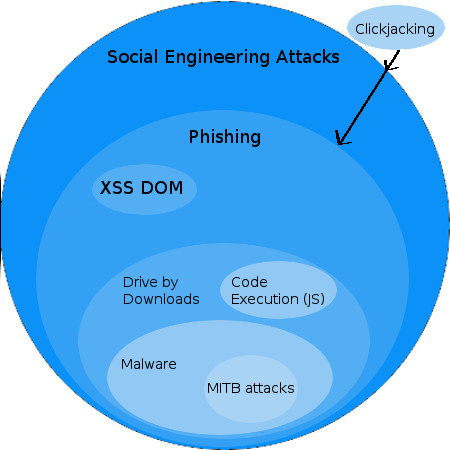
\includegraphics[scale=0.6]{figures/SEAttacks.jpg}
        \caption{Esquematización de ataques de tipo Social Engineering.}
        \label{fig:SEattack}
    \end{figure}

\subsection{Análisis de ataques}
    Según los estudios \cite{browSecPhish, Labs2013, rowSecSEMBlock} indican que el \textit{Browser} es la primera linea de defensa en contra de multiples amenazas en la Web. Sin embargo, esto se ve afectado bastante por la falta de educación de los usuarios que utilizan los navegadores y la constante evolución de las amenazas \cite{browSecPhish} Es por esto que muchos de los manufacturadores de browsers crean mecanismos de defensa \cite{Drake2011} que actuen al momento de solicitar una página, usando black o white list, sistemas de reputación \cite{Rajab2013} con avisos de alerta al usuario, para evitar que éste al menos tome la decisión de poder ingresar al sitio malicioso.

\subsection{Phishing}
Este ataque consta principalmente del engaño al usuario, confundiéndolo a que visite una página deshonesta en vez de la que tenía pensado. En el último tiempo muchos de los ataques que actualmente están ocurriendo se han limitado al uso de técnicas de ingeniería social. Si bien los ataques basados en drive-by downloads y clickjacking siguen siendo de alto impacto, los atacantes parecen preferir los otros por la simplicidad de éste, pues no es necesario conocer realmente vulnerabilidades del \textit{Browser} para llevarlos a cabo. Sin embargo, el Phishing es una buena herramienta que permite generar muchos otros ataques, que son mucho más peligrosos. Un resultado obtenido dentro del experimento en \cite{browSecPhish}, menciona que la vida útil en promedio de un sitio de Phishing es de aproximadamente 26 horas. Esto principalmente es debido a que los sistemas de defensa, antes de saber si es malicioso o no, debe descubrir, validar y clasificar en el Sistema de Reputación, tan pronto como sea posible. Un ataque de Phishing puede tener los siguientes ataques asociados:

	\subsubsection{Instalación de Malware o Extensiones malignas}
	Un ataque de éste tipo puede ser originado desde la ejecución de un ataque Phishing a una persona; en especial cuando se hace creer que lo que se va a instalar es completamente inofensivo. Sin embargo, el resultado de la aceptación de usuario a la instalación puede tener consecuencias bastante graves, tanto en el Browser como en el Host, donde la mayoría de las veces el ataque puede terminar como un Man-in-the-Browser \cite{Utakrit2009, Dougan2012}. En la jerga de NSS Labs estos ataques son llamados SEM (Social Enginerring Malware), en el estudio \cite{rowSecSEMBlock} afirma que conocer la identidad de los atacantes que utilizan Social Engineering permite una mejor protección contra los SEM. El trabajo recomienda que las empresas y grandes organizaciones deberían revisar los reportes de otros Laboratorios de Seguridad cuando seleccionan un tipo de Web Browser; Las empresas deben entender que el mercado de los Browsers no es estático y muchas amenazas aparecen constantemente. El estudio concluye que la Educación es un componente importante en la protección de SEM, pues aquellos usuarios que son capaces de identificar ataques de Ingeniería Social (SE), necesitan menos tecnologías para la protección de estos ataques.

	\subsubsection{Extensiones vulnerables}
	Muchas veces un ataque Phishing se aprovechará de las extensiones \textit{benign-but-buggy}; extensiones que tienen un propósito benigno para el usuario que las usa, pero que un atacante puede aprovecharse de alguna vulnerabilidad \cite{Barth2010, Liu2012}. Además dependiendo del tipo de arquitectura que el Browser pueda tener, es posible que el atacante utilice una extensión que tenga permisos a ciertos recursos del Host o que pueda coludirse con otra extensión benigna para lograr un ataque en forma conjunta \cite{Saini2014}; donde lo peor de todo, es que el tráfico no será detectado como malicioso.

	\subsubsection{Ejecución de Código Javascript}
    Este tipo de ataques ocurren cuando es posible ejecutar un script en el interprete del cliente, de manera que pueda generar acciones maliciosas dentro del Browser del Cliente. Este tipo de ataque funciona muy bien, cuando el atacante desea que el Web Browser de la víctima realice acciones en nombre del atacante, de tal manera que la identificación de éste se haga casi imposible. En ciertas situaciones un atacante podría aprovecharse de alguna vulnerabilidad asociada a los modelos de seguridad que Javascript y DOM poseen, pues ambos son totalmente transversales. Javascript utiliza un modelo de seguridad en sus objetos basado en \textbf{Capabilities}, mientras que DOM refuerza el \textbf{Same Origin Policy} por medio del uso de un \textbf{Reference Monitor} para controlar el acceso de código de diversos \textbf{orígenes}. Es en esta situación donde podría llevarse a cabo la ejecución de código javascript, aún cuando éste pueda ser de un \textbf{origen} distinto al receptor \cite{Barth2009}.

	\subsubsection{XSS DOM - Cross-Site Scripting DOM}
	Es un ataque XSS en donde su \textit{payload} de ataque es ejecutado como resultado de la modificación del \textit{ambiente} DOM en el navegador de la víctima usado por el código script original; en consecuencia el código de cliente se ejecuta de una manera inesperada. El ataque Cross-Site Scripting (XSS) normalmente se asocia con ataques que afectan directamente al servidor, pero existe una tercera variedad que afecta directamente al navegador \cite{Singh2014} y que puede ser tan peligrosa como su forma \textbf{Reflejada} o \textbf{Almacenada}, ésta es llamada XSS DOM o \textbf{tipo-0 XSS} \cite{XSSDOMOwasp, XSSDOM}. Un ejemplo de un simple XSS DOM puede verse en \cite{bugzillaXSSDOM}. Un UXSS o Universal XSS es un ataque más particular, y tiene la habilidad de ser gatillado al explotar una falla en el interior del Browser \cite{Paola2006}, a diferencia de otros XSS que buscan la vulnerabilidad dentro de la Aplicación Web con el que se comunican.


	\subsubsection{Man in the \textit{Browser} (MitB)}
    Un Man in the Browser es una técnica utilizada por un atacante para poder leer o modificar datos que se envían entre el cliente Web y el Servidor que responde a las \textit{request}. La diferencia sustancial entre un Man in the Browser (MitB) y un Man in the Middle (MitM) es el dominio que ataca, el primero es al nivel de la capa de aplicación, mientras que el segundo tiene que ver más con el canal de comunicación. \cite{Dougan2012} explica las grandes diferencias entre estos dos ataques, donde principalmente un MitB se inicia con un ataque Phishing que logra convencer al usuario de instalar alguna extensión o ejecutar una pieza de código \cite{Utakrit2009, Paola2006}, que permita al atacante estar entre el Browser y el Host, de tal manera que todas las solicitudes pueden ser escuchadas y modificadas dentro del mismo Host.




%\section{Mecanismos de Defensa del Host}
%	Dependiendo del Sistema Operativo, es posible encontrar diversos mecanismos de Defensa. Tanto Linux como Windows poseen mecanismos parecidos, donde se diferencia la implementación. Dado que la mayor parte de los usuarios en internet usan Windows (Figura \ref{fig:OS}) nos enfocaremos en éste para mostrar los mecanismos implementados en el Host.

%	\begin{figure}[h!t]
 %       \centering
  %      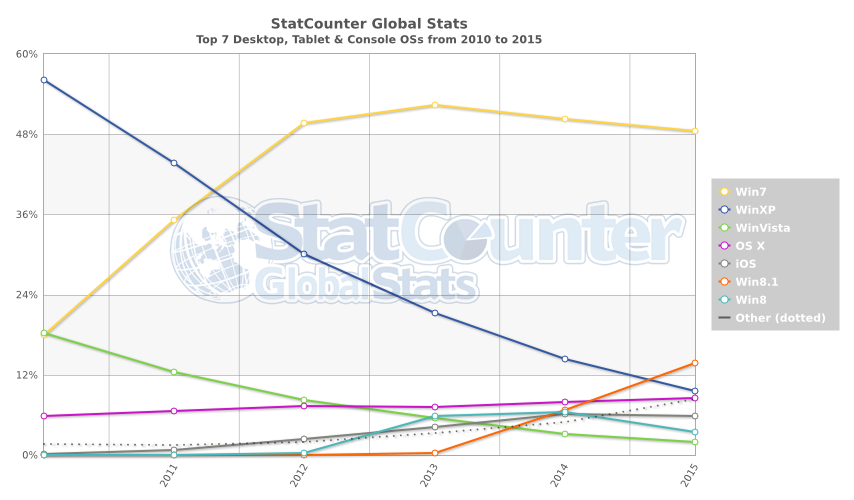
\includegraphics[scale=0.5]{figures/StatCounter-os-ww-yearly-2010-2015.png}
   %     \caption{Gráfico con porcentaje de tipo de sistemas operativos más usados. Fuente: \cite{statOS}}
    %    \label{fig:OS}
    %\end{figure}

    %\subsection{DEP/NX o Data Execution Prevention}

    %\subsectiob{ASLR o Address Space Layout Randomization}

    %\subsection{/GS (Buffer Security Check)}

    %\subsection{SafeSEH}

    %\subsection{Function Pointer Ofuscation}

    %\subsection{Export Address Table Access Filtering (EAF)}

    %\subsection{NULL page allocation}


\section{Mecanismos de Defensa del \textit{Browser}}

\subsection{SOP: Same Origin Policy} %listo
\label{chap2:SOP}

    Es un principio de seguridad implementado (hoy en día) por cada browser existente, su principal objetivo es restringuir las formas de comunicación entre una ventana y un servidor web. \textbf{Same Origin Policy} o \textbf{SOP} es un acuerdo entre varios manufacturadores de navegadores web como Microsoft, Apple, Google y Mozilla (entre los más importantes), en donde se definió una estandarización de cómo limitar las funcionalidades del código de \textit{scripting} ejecutado en el browser del usuario \cite{SOPIEFT}. 

    Este importante concepto nace a partir del Modelo de Seguridad detrás de una Aplicación Web, al mismo tiempo que es el mecanismo más básico que el Browser tiene para protegerse de las amenazas que aparecen en el día a día, haciendo un poco más complicado el trabajo de crear un \textit{exploit}. \textbf{SOP} define lo que es un \textbf{Origen}, compuesto por el \textbf{esquema}, el \textbf{host/dominio} y \textbf{puerto} de la URL. Esta política permite que un Web Browser aisle los distintos recursos obtenidos por las páginas web y que solo permita la ejecución de \textit{Scripts} que pertenezcan a un mismo \textbf{Origen}. Inicialmente fue definido solo para recursos externos, pero fue extendido para incluir otros tipos de orígenes, esto incluye el acceso local a los archivos con el \textit{scheme} \textbf{file://} o recursos relacionados al Browser con \textbf{chrome://}.

    \textbf{SOP} puede distinguir entre la información que envía y recibe el Web Browser, y solo se aplicará la política a los elementos externos que se soliciten dentro de una página web (recepción de la información). Esta imposibilidad de recibir información de un \textbf{Origen} diferente al del recurso actual, permite disminuir la superficie de ataque (\textit{Attack Surface}) y la posibilidad de explotar alguna vulnerabilidad en el sistema donde reside el Browser. Sin embargo, \textbf{SOP} no pone ninguna restricción sobre la información que el usuario puede enviar hacia otros. Sin \textbf{SOP} cualquier sitio podría acceder a la información confidencial de un usuario o de cualquier otro sitio. Por tanto es sencillo entender la razón de la existencia de \textbf{SOP}, se desea proteger la información del usuario, sus cookies, token de autenticación, etc. de las amenazas existentes en la Internet.


    %referencia de chrome Zalewsk08
    En \cite{Zalewsk08} se menciona que no existe una sola forma de \textbf{SOP}, si no que es una serie de mecanismos que superficialmente se parecen, pero al mismo tiempo poseen diferencias:

    \begin{itemize}
        \item \textbf{SOP} para acceso al \textbf{Document Object Model}: se dará permiso de modificar el \textbf{DOM} y sus propiedades solamente aquellos scripts que tienen el mismo dominio, puerto (para todos los browsers excepto Internet Explorer) y protocolo. Visto de otro modo, el mecanismo entrega una especie de Sandboxing para el contenido potencialmente peligroso y no confiable. Sin embargo, éste no es suficiente, pues posee varias desventajas: el dominio es posible de cambiar a la conveniencia del atacante, limita las acciones a los desarrolladores, lo que se traduce en que éstos tengan que buscar bugs que permitan liberarse de estas restricciones, lo que incita a atacantes a aprovecharse de esto.
        \item \textbf{SOP} para el objeto XmlHttpRequest: para diferentes tipos de peticiones (GET, POST y otros) existen condiciones y suposiciones que hacen que se tome o no en cuenta el \textit{request} del cliente, además del uso de una \textit{whitelist} de las formas en que el header de la petición puede salir del browser.
        \item \textbf{SOP} para \textit{cookies}: restringuiendo el uso de acuerdo su dominio, \textit{path}, tiempo de uso, modificando o eliminado las cookies, e incluso protegiendo las cookies usando el \textit{keyword: secure}. Sin embargo, desde su implementación las cookies han generado bastante problemas de seguridad.
        \item Y otros como: {SOP} para Flash, donde usa políticas para realizar peticiones fuera del dominio através de un archivo \textbf{crossdomain.xml}, \textbf{SOP} para Java y \textbf{SOP} para Silverlight, parecido al de Flash solo qe utiliza otros elementos.
    \end{itemize}

    
    Tanto para los atacantes como desarrolladores de Software, SOP puede llegar a ser bastante molesto. Para el primero, la respuesta es obvia, pero para el segundo está el problema de ¿cómo poder aislar los componentes no confiables o parcialmente confiables, mientras que al mismo tiempo se pueda tener una comunicación entre ellos de forma segura? Ejemplo de esto son los Mashup \cite{barth2009securing}, que permiten juntar contenido de terceros en una misma página por medio de frames, etc. 
        
    Existen excepciones que permiten evitar el uso de SOP, pero como es de esperar esta vía puede ser mal usada por los atacantes en contra del usuario y de la Aplicación Web. Dentro de las excepciones están los elementos en HTML \(<\)script\(>\), \(<\)img\(>\), \(<\)iframe\(>\) y otros, que si bien permiten la comunicación entre diferentes orígenes, un mal uso de éste puede causar grandes estragos, desde la eliminación de registros en una base de datos hasta la propagación de un gusano o virus.
        
    Queda decir que si bien SOP entrega una capa de seguridad al usuario y a la Aplicación Web, contra cierto tipo de ataques (muchas veces del tipo de ataques de principiantes), esto no es suficiente. Es responsabilidad del desarrollador de Software poseer las herramientas necesarias para asegurar la confidencialidad e integridad del sistema a través de otros métodos de seguridad.



\subsection{CORS: Cross-Origin Resource Sharing}
\label{chap2:CORS}
    Cómo lo define su nombre, es un mecanismo (especificación) que permite al cliente realizar peticiones entre sitios de diverso \textbf{Origen u Origin}, ignorando el \textbf{SOP}. \textit{CORS} define una forma en que el Browser y el Servidor Web puedan interactuar para determinar si permitir o no la petición a otro \textbf{Origen}. Un Browser utiliza SOP para restringuir las peticiones de la red y prevenir al cliente de una Aplicación Web ejecutar código que se encuentra en un origen distinto, además de limitar los \textit{request} HTTP no seguros que podrían tratar de generar un daño. CORS extiende el modelo que el Browser maneja e incluye:
        
        \begin{itemize}
            \item Un campo en el header de la respuesta/\textit{response} del servidor solicitado llamado \textit{Access-Control-Allow-Origin}, donde se debe escribir el \textbf{Origen} que tendrá acceso a los recursos solicitados al servidor. Si el valor de la respuesta del servidor coincide con el \textbf{Origen} de quien lo solicitó, se podrá realizar el uso del recurso en el navegador, de lo contrario se generará un error.

            \item Otro campo llamado \textbf{Origin}, pero esta vez en la cabecera de la solicitud, para permitir al Servidor hacer cumplir las limitaciones en las peticiones de distinto \textbf{Origen}.

            \item En algunos casos un browser deberá agregar en el header el campo \textit{Access-Control-Allow-Methods}, ya que el servidor no responderá de vuelta si no es así. Esto permite limitar la superficie de ataque en el servidor.

        \end{itemize}
    Existen ciertos métodos en HTTP que necesitan realizar un \textit{pre-vuelo} antes de ser ejecutados, si la respuesta/\textit{response} del servidor es afirmativa luego se enviará la peticióm original con el método que se debió confirmar su utilización. Para el caso de los métodos GET y POST, los más usados, este pre-vuelo no es necesario y se puede enviar la petición/\textit{request} inmediatamente.
    
    La gran diferencia de CORS con cualquier otro método es que permita hacer peticiones hacia un \textbf{Origen} distinto, es que el Browser por omisión no enviará ningún tipo de información que permita identificar al usuario. De esta manera se puede disminuir considerablemente las amenazas en la confidencialidad, pues el atacante no podrá hacerse pasar por un usuario del que no tiene información. Casi todos los navegadores web, a diferencia de Internet Explorer \cite{bookWebAppSec}, realizan sus solicitudes a servidores de diverso \textbf{Origen} por medio de la interfaz \textit{XmlHttpRequest}, en el caso de Internet Explorer esta se llama \textit{XDomainRequest}.

\subsection{HTTP Fields/Campos HTTP}
    \label{chap2:headers}
    HTTP es un protocolo de la capa de aplicación del modelo OSI, que todo dispositivo debe seguir si desea conectarse a la Internet. El \textit{header} o cabecera que utiliza este protocolo permiten configurar la comunicación entre un \textit{Web Server} y un cliente web, en este caso con el Browser. Estos campos del \textit{header} indican \textbf{dónde} debe ir el mensaje y \textbf{cómo} deben ser manejados los contenidos del mensaje. En cada petición o \textit{request} del Navegador, éste debe especificarlos para que el servidor pueda enteder las peticiones; de la misma manera, el servidor enviará una cabecera con campos que el cliente también debe entender. Algunos campos son necesarios y hasta obligatorios, para algunos servidores, y en otros da lo mismo como vayan.

        \begin{itemize}
            \item Content Security Policy Flag: Es un mecanismo de defensa creado exclusivamente para la defensa de ataque de tipo XSS o \textit{Cross-Site Scripting}. La misión de éste es definir bien la línea entre intrucciones y contenido, donde la primera se refiere a código que se debe ejecutar. Para que sea posible utilizar este mecanismo es necesario agregar a la cabecera del servidor, en la petición del cliente, el campo Content-Security-Policy o X-Content-Security-Policy, donde se indica la localización de donde los scripts pueden ser obtenidos o \textit{loaded} y además pone restricciones a estos mismos scripts.

            \item Secure Cookie Flag: El propósito de este campo es de instruir al Browser de nunca mandar una \textit{cookie} sobre un canal no seguro, solo debe ser realizado por HTTPS. Esta medida permite asegurar que una cookie tampoco será enviada por canales mixtos, donde al inicio de la comunicación HTTPS y luego vuelve a HTTP.

            \item HttpOnly Cookie Flag: Una opción para las \textit{cookies} que permite inhabilitar el acceso al contenido de una cookie por medio de scripts. Esta opción originalmente fue pensada para evitar ataques XSS.

            \item X-Content-Type-Options: Un servidor que manda la directiva nosniff para en la cabecera/\textit{header}, obligará al Browser a renderizar la página así como lo dice el campo content-type. La idea de este \textit{flag} es poder limitar la ejecución del tipo objeto que pide el browser.

            \item Strict-Transport-Security \cite{RFC-6797}: Obliga al navegador a que la comunicación con el servidor sea realizada por un tunel válido HTTPS, de manera que la comunicación sea completamente segura.

            \item X-Frame-Options: este campo previene que se realize un \textit{framing} de la página, es decir, esta opción evita que la página sea mostrada a través de un \(<\)iframe\(>\). Este control permite especialmente mitigar ataques de \textit{Clickjacking}, donde el usuario es engañado a través de lo que se muestra en la ventana del navegador.
        \end{itemize}

\subsection{Sandboxing}
    \label{chap3:Sandboxing}
    La idea es encapsular el área de mayor probabilidad de ataque en un espacio aislado, minimizando la superficie de ataque de un software. Sandboxing no es una técnica tan nueva, han existido sistemas que ya lo han incorporado. Ésta protección puede ser aplicada dependiendo del diseño del software, algunos ocupan Sandbox a nivel del sistema operativo como otros que ocupan al nivel del \textit{engine} de Javascript \cite{reis2009browser}. En el caso especial del \textit{Browser}, esta técnica es construida en el nivel más alto posible para un programa de usuario, lo que permite la separación de privilegios entregados por el sistema operativo al \textit{browser} y los subprocesos que corren dentro de éste. El atacante que se enfrente a un \textit{browser} que tenga este mecanismo de defensa, tendrá que realizar primero un \textit{bypass}, encontrando una vulnerabilidad en el sandboxing del \textit{browser}. Existen diferentes técnicas para Sandboxing, todo depende del diseño del \textit{Browser}.

    En el desarrollo de Chromium \cite{barth2008security} se define un modelo de amenazas donde enumeran las habilidades que debería de tener un atacante y los objetivos de estos, para así caracterizar y evaluar las propiedades de seguridad necesarias para evitar que los atacantes cumplan su objetivo. Una propiedad importante que hacen destacar en el estudio es cómo aislar ciertos procesos que pueden ser aprovechados por los atacantes y ofrece una forma para poder mitigar esto: Sandboxing. El Sandboxing de Google Chrome previene al atacante de leer o escribir en el sistema de archivos del usuario, dejando al \textit{Principal Web} con los privilegios necesarios para parsear un HTML/XML y ejecutar código JavaScript. Sin embargo esta arquitectura no imposibilita al atacante a atacar otros sitios web si es que el Rendering Engine fue comprometido, lo que puede convertirse en una amenaza muy grande para otros sitios web.

    Mientras Google Chrome e Internet Explorer utilizan un Sandbox para sus procesos de renderizado/\textit{rendering} \cite{sandboxGC}, Firefox no ha realizado este trabajo ni siquiera en su versión monoproceso \cite{NeckoElectro}.



    \subsubsection{Google}
        El Sandbox de Google es una implementación propia y que también aprovecha las técnologías disponibles en el Sistema Operativo. La idea del Sandbox es restringuir el acceso o peticiones al sistema de archivos, de modo que la única manera es pidiendo a otro que realice el trabajo que el proceso dentro del Sandbox necesita.

        \begin{figure}[h!t]
            \centering
            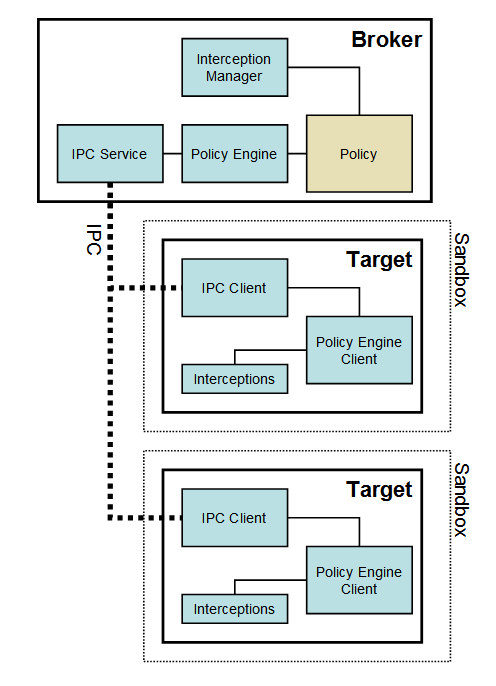
\includegraphics[scale=0.5]{figures/sbox_top_diagram.png}
            \caption{Sandbox interno de Google Chrome/Chromium. Fuente: \cite{sandboxGC}}
            \label{fig:SandboxGC}
        \end{figure}

    \subsubsection{Internet Explorer}
        Un nuevo mecanismo para aislar procesos es introducido en Windows 8, llamado AppContainer, es el principal mecanismo usado por Enhanced Protected Mode para aislar y limitar los privilegios y capacidades de un proceso con Sandboxing.
        \begin{figure}[h!t]
            \centering
            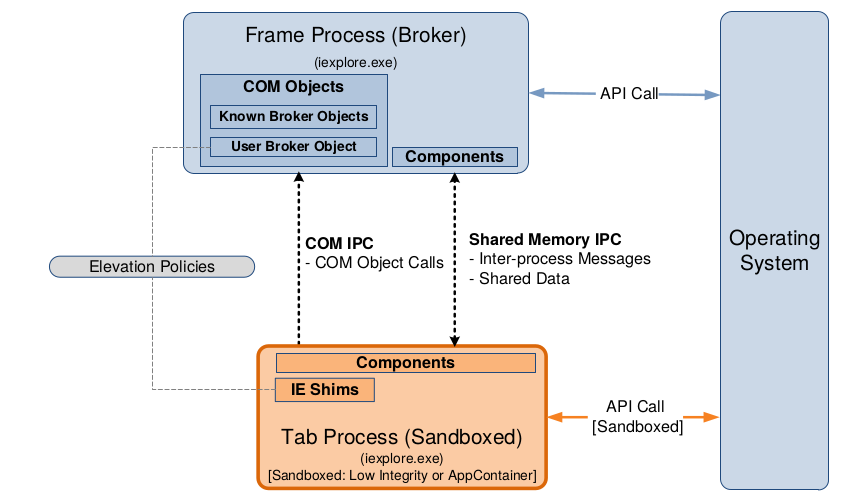
\includegraphics[scale=0.5]{figures/sandboxIE.png}
            \caption{Sandbox interno de Internet Explorer. Fuente: \cite{Yason}}
            \label{fig:SandboxIE}
        \end{figure}

        \begin{figure}[h!t]
            \centering
            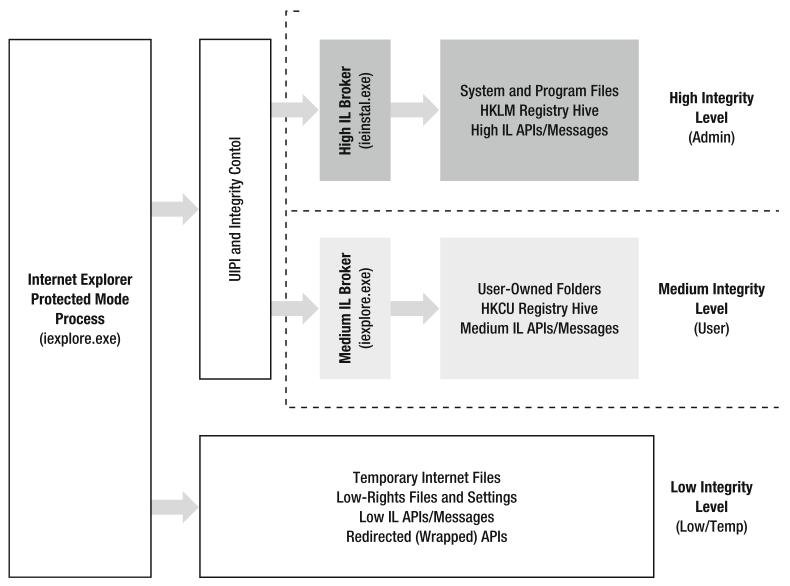
\includegraphics[scale=0.5]{figures/IEProtectedMode.jpg}
            \caption{Sandbox, Protected Mode. Fuente: \cite{Crowley2010}}
            \label{fig:SandboxIE2}
        \end{figure}
        La idea principal del Sandboxing en IE es restringuir el acceso de escritura a objetos \textit{asegurables}, como procesos, archivos o llaves de registro que sean de niveles de integridad mayor \cite{Colvin2010}. El proceso mismo de Internet Explorer posee un nivel de integridad baja, por lo tanto la única manera de modificar algo es cuando se le pregunta explícitamente al usuario y éste lo permite.



 \subsection{Aislación de Contenido}
    Cuando hablamos de Aislación de Contenido, nos referimos a cómo los Navegadores realizan la separación del contenido que será renderizado. Esto es dado que si no se es cuidadoso, scripts de otro \textbf{Origen} podrían intervenir con una página benigna y tomar control de ésta. Google Chrome aisla el contenido de cada recurso que el usuario pide, por medio de la instanciación de \textit{siteinstance-per-process} \cite{Reis2009}, aunque durante este último tiempo están tratando de mejorarlo a \textit{site-per-process} \cite{GoogleChromeIsolation}. Esto último significaría que cada página y \textit{frame} tendría su propio proceso, separando completamente los espacios de memoria que cada componente de la página usaría al ser renderizada. Esto permite disminuir tanto la superficie de ataque, como incrementar la estabilidad del Browser, si es que algún componente provoca algún fallo. Firefox \cite{FirefoxThreatModel}, por su parte, promete que en futuras versiones del Browser multiproceso, diferentes \textit{Tabs} podrán correr en diferentes procesos de acuerdo a su dominio, pero por ahora todas las tabs de contenidos comparten un solo process de \textit{Content process}.

    La Aislación de Contenido es importante pues permite proveer de Seguridad, Sensibilidad, Estabilidad y Confiabilidad. Por ejemplo, si el Browser utiliza un enfoque en que separa el contenido al igual que Google Chrome, cada proceso tendrá su espacio de memoria, lo que permite implementar medidas como ALSR \cite{Drake2011}, para que los espacios de memoria sean \textit{random} cada vez que se cree un nuevo proceso. Al separar en procesos, se están crendo distintas tareas que el sistema operativo se encargará de distribuir y computar de forma paralela; por lo que si alguno de estos procesos se cae, el proceso principal y todos los asociados, no deberían de ser afectados. Con Internet Explorer no se ha podido observar qué tipo de separación de contenido posee, pero debe ser algo parecido a Google Chrome y Firefox.
    
    Uno de los pasos que ha tomado Google Chrome/Chromium y que Firefox va para el mismo rumbo con la API \textbf{WebExtension} \cite{AddONFirefox}, es la aislación de las extensiones del contenido de la página, tal como lo sugiere \cite{Barth2010}. Donde un \textit{Content script} es el que podrá cambiar el contenido del DOM, pero no será capaz de afectar a las Tabs, Bookmarks de otro Tab y menos el sistema de archivos, a excepción que encuentre una vulnerabilidad que se lo permita.
    
    %GC: Barth2010, Barth2009SecureFrame, Reis2009, barth2008security
    %IE: Crowley2010, Yason
    %Todo: Drake2011, Saini2014, Silic2010

 \subsection{Blacklist y Whitelist de sitios web}

    El estudio \cite{browSecPhish} explica las más comunes y efectivas amenazas de seguridad que los usuarios hoy en día se enfrentan, entre ellas están el Software Engineering Malware y el Phishing. Un experimento es llevado a cabo en este estudio, con evidencia empíricamente validada y obtenida por NSS durante 12 días de continuo testing. Se obtuvo como resultado que Safe Browsing de Google Chrome provee una mejor protección contra ataques de tipo Phishing, si es comparado con SmartScreen de Internet Explorer. Estos mecanismos poseen habilidad para alertar a la posible víctima, de  que están a punto de pedir un recurso que puede ser malicioso. Una de las conclusiones del estudio de NSS Labs \cite{rowSecSEMBlock} es que afirma que la tecnología de Google Safe Browsing no provee una protección adecuada para SEM\footnote{Social Engineering Malware}, pero tecnologías basadas en CAMP\footnote{Content-Agnostic Malware Protection} ayudan bastante.

    Tanto Google como Firefox usan Safe Browsing para investigar si un cierto recurso, detrás de la URL pedida, es posible que se trate de un Phishing. Ambos tienen listas negras que se van actualizando muchas veces en el día, el menos 2 veces por hora. Esto permite disminuir la cantidad de ataques de este tipo, pero lamentablemente el dinamismo de este tipo de ataque a veces hace imposible tener una lista de todos los sitios manipulados.

    El trabajo que explica CAMP \cite{Rajab2013}, utiliza una Whitelist dentro del Cliente Web para limitar la cantidad de peticiones que recibe el Sistema de Reputación desde todos los Navegadores que necesitan información sobre un binario, que posiblemente pueda ser SEM.
        %GC y Firefox
    Internet Explorer utiliza URL Filtering, con el SmartScreen, que permite obtener una buena protección contra SEM \cite{rowSecSEMBlock} a diferencia de los otros manufacturados de navegadores.
    %\cite{Crowley2010, Colvin2010}

 \subsection{Sistemas de Reputación}
    %Agregar que estos s complementar con blacklist y a veces whitelist (GC)
    Cada vez que un usuario desea un recurso, por medio de su URL, el usuario podría no saber que detrás de ese \textit{path} puede haber una amenaza. Un Sistema de Reputación trabaja en base a los distintos tipos de binarios que un usuario podría llegar a descargar, ya sea un archivo muy descargado que podría estar disfrazado como una imagen y en verdad se trata de un virus, o simplemente un pdf que es descargado por un grupo de alumnos de un curso con poca concurrencia. La idea detrás es tener un sistema centralizado que se encarga de dar una \textbf{reputación} al binario, dependiendo de la técnica usada. Tanto Internet Explorer como Google Chrome utilizan este tipo de sistema, pero cada uno lo implemente de distinta manera. Un buen sistema basado en Reputación es aquel que es preciso y rápido, de manera que sea posible de obtener altos porcentajes de detección (efectividad).

    El estudio realizado por NSS Labs \cite{rowSecSEMBlock}, hizo una experimentación de la capacidad de detección y bloqueo de Malware en los Browser más conocidos, entre ellos Firefox, Internet Explorer y Google Chrome. Se usaron 657 muestras de SEM, que fueron capturados por el laboratorio dentro de 14 días. Los ataques basados en SEM usan diferentes métodos para poder engañar a los usuarios. Uno de los puntos que dejan claro, es que el factor primario es el Web Browser, dado que es la primera línea de defensa de los usuarios en contra de la mayoría de los ataques SEM. El test realizado dentro de la experimentación demostró que Internet Explorer bloqueaba casi un \(99,9\%\) de los SEM sacados de la muestra usadas dentro del test. Google Chrome le sigue a IE con la mejor detección de Malware y otros Browser con tecnologías basadas en Cloud (KingSoft Antivirus), generan una mejor detección que Firefox (\(4,2\%\)). La alta detección y bloqueo obtenido tanto por Internet Explorer y Google Chrome/Chromium, es gracias a las tecnologías SmartScreen URL Filtering (filtro de URL, como black list) y Application Reputation, Chrome por su parte usa Safe Browsing API y Download Protection para resguardarse. Sin embargo, Internet Explorer no depende tanto en su Sistema de Reputación así como lo realiza Google Chrome, donde el \(2,9\%\) del \(99,9\%\) de la detección de IE es basada en la técnología CAMP y Google Chrome detecta \(66,5\%\) del \(70,7\%\) con su Download Protection. Ésto último significa para Google Chrome/Chromium, que su sistemas de Reputación es su mejor protección contra Malware. 

    %\subsubsection{Google Download - Google Chrome/Chromium}
        %Ocupar referencias de NSS para los resultados obtenidos
    %\subsubsection{SmartScreen - Internet Explorer}


 %\subsection{Filtros XSS}
  %  Los Filtros XSS son una medida preventiva contra posibles ataques XSS insertados en la response del servidor. Principalmente se encarga de prevenir XSS de tipo Reflejado o Almacenado, pues los tipo DOM podría ocupar técnicas para 
    %Google e IE
    %Firefox ocupa 3rd party
    %Vulnerabilidades mencionadas \cite{Bates2010}y la solución del paper es crear un filtro que detenga los ataques antes de que sean interpretados por el Renderer
 %\subsection{Safe Sanitization}

 %\subsection{AdBlocker}

 \subsection{Actualizaciones Periódicas en Background}
 Tanto Google Chrome \cite{reis2009browser} como Firefox realizan actualizaciones automáticas periódicas del Navegador, para reducir la ventana de posible vulnerabilidades que pueda tener una versión. Parte importante de esto es que este proceso no fastidia al usuario y permite que se instale apenas el browser se cierra, para que en la próxima sesión sea posible usar la nueva.

